\section{Elektronischer Aufbau}
\label{sec:Elektronik}
Um ein gesamtes funktionsfähiges Mess- und Verarbeitungssystem realisieren zu können, sind mehrere Schritte, hinsichtlich des mechanischen und elektronischen Aufbaus notwendig. Dazu zählen unter anderem die Wahl der Hardwareplattform, die Auslegung eines Spannungsversorgungssystems und Möglichkeiten, den Zustand des Programmes erkennen und ändern zu können. Außerdem ist ein robustes Gehäuse zur Einhausung dieser Komponenten sowie mehrerer Sensoren zu konstruieren und fertigen. Zusätzlich sind externe, im Gehäuse nicht verbaute Sensoren, über eine zuverlässige Verbindung in das Elektroniksystem einzubinden.

\subsection{Wahl der Hardware-Plattform}
\label{subsec:elekMikrocontroller}
An die Hardware-Plattform werden einige Anforderungen gestellt. Sie muss Möglichkeiten zur Kommunikation mit den Sensoren bieten, außerdem muss sie genug Rechenleistung aufbringen können, um alle Sensoren simultan auszulesen und diese Daten für die spätere Verwendung aufzuzeichnen. Es sollten außerdem Optionen vorhanden sein, die gesammelten Daten vom ferngesteuerten Auto zu exportieren, um sie auf einem anderen Gerät auszuwerten. Eine weitere essentielle Eigenschaft ist, in welchen Programmiersprachen die Hardware programmiert werden kann, da die Verfügbarkeit von Bibliotheken für die jeweilige Programmiersprache eine wichtige Rolle spielt. Andere Faktoren, die zwar nicht notwendig sind, aber von großem Nutzen sein können, sind \ac{WLAN}- und Bluetooth-Funktionalität. Die bekanntesten Hersteller von solchen Plattformen sind Raspberry Pi und Arduino.  Beide Hersteller bieten sowohl größere und leistungsstärkere als auch kleinere, leistungsschwächere Optionen an. Die bekanntesten Optionen sind somit der Raspberry Pi 4 Model B, der Raspberry Pi Zero 2 W, der Arduino Uno und der Arduino Nano.
\begin{table}[h]
\centering
\begin{tabular}{|c||c|c|c|c|} 
\hline
Plattform                                                      & Arduino Uno                                                                                 & Arduino Nano                                                                                & Raspi 4B                                                                                           & Raspi Zero 2 W                                                                             \\ 
\hhline{|=::====|}
Prozessor                                                      & ATmega328P                                                                                  & ATmega328                                                                                   & BCM2711                                                                                            & Cortex-A53                                                                                \\ 
\hline
Schnittstellen                                                 & \begin{tabular}[c]{@{}c@{}}UART\\SPI\\I$^2$C\\6 analoge Pins\\14 digitale Pins\end{tabular} & \begin{tabular}[c]{@{}c@{}}UART\\SPI\\I$^2$C\\8 analoge Pins\\12 digitale Pins\end{tabular} & \begin{tabular}[c]{@{}c@{}}UART\\SPI\\I$^2$C\\28 GPIO Pins \\4 USB Ports\\RJ45 Buchse\end{tabular} & \begin{tabular}[c]{@{}c@{}}UART\\SPI\\I$^2$C\\28 GPIO Pins \\micro USB Port\end{tabular}  \\ 
\hline
\begin{tabular}[c]{@{}c@{}}Programmier-\\sprachen\end{tabular} & C, C++                                                                                      & C, C++                                                                                      & \begin{tabular}[c]{@{}c@{}}Python\\C, C++\\Scratch\end{tabular}                                    & \begin{tabular}[c]{@{}c@{}}Python\\C, C++\\Scratch\end{tabular}                           \\ 
\hline
\begin{tabular}[c]{@{}c@{}}Zusatz-\\funktionen\end{tabular}    & -                                                                                           & -                                                                                           & WLAN, Bluetooth                                                                                    & WLAN, Bluetooth                                                                           \\ 
\hline
Preis                                                          & 20\officialeuro                                                                                                                                                                                   & 18\officialeuro                                                                                          & ab \$35                                                                                            & \$15                                                                                      \\
\hline
\end{tabular}
\caption{Vergleich von verschiedenen Hardware-Plattformen}
\label{tab:myCcomparison}
\end{table}
\\
Da auf dem Raspberry Pi wie in Sektion \ref{subsec:tRasPiOS} beschrieben eine vollwertige Linux-Distribution läuft, können auf Einplatinencomputer von Raspberry Pi alle programmiersprachen verwendet werden, die unter Linux unterstützt sind. Die in der Tabelle aufgelisteten Sprachen sind die, die von Raspberry Pi OS standardmäßig unterstützt werden, ohne eigens Pakete installieren zu müssen.\\
Aufgrund der im Vergleich zum ATmega328 hohen Rechenleistung des Arm Cortex-A53, der Option, Einplatinencomputer von Raspberry Pi mit Python zu programmieren, der zusätzlichen \ac{WLAN}-Funktion und den niedrigen Preises wird der Raspberry Pi Zero 2 W verwendet. Ein weiterer Vorteil des Raspberry Pi ist es, dass er einen eingebauten microSD Kartenslot hat, die damit verwendete microSD Karte dient als Hauptspeicher des Einplatinencomputers. Dieses Speichermedium kann deswegen auch gleich für das Aufzeichnen der Daten verwendet werden, somit entfällt die Notwendigkeit für ein externes SD-Kartenmodul, welches bei einem Arduino notwendig wäre.

\subsection{Spannungsversorgung}
\label{subsec:elekSupply}
Da das Auto, wie in Sektion \ref{sec:Auto} beschrieben, mit zwei 7.4\ac{V} Lithium Polymer Akkus betrieben wird, bietet sich die Möglichkeit an, diese auch für die Versorgung der Messelektronik zu verwenden. Um die Akkus gleichmäßig zu belasten werden beide in Serie geschalteten Akkus für diese Spannungsversorgung verwendet. Damit stehen 14.8\ac{V} zur Verfügung, welche mit einem DC-DC Stepdown-Converter auf 5\ac{V}, was der Versorgungsspannung des Raspberry Pi entspricht, herabgewandelt werden. Der DC-DC-Converter weist am Eingang zwei Schraubklemmen sowie eine Hohlbuchse auf. Die Leitungen der Akkus werden an den Schraubklemmen am Eingang des Converters angeschlossen. Ein Kippschalter, der die Plus-Leitung unterbrechen kann, ermöglicht das manuelle Aus- und Einschalten der gesamten Messelektronik. Zusätzlich wird ein Voltmeter mit Siebensegmentanzeige an der Hohlsteckerverbindung am Eingang angeschlossen, welches die Akkuspannung anzeigt (Siehe Abbildung \ref{fig:switch}). Der Stepdown-Wandler weist am Ausgang ebenfalls zwei Schraubklemmen und zusätzlich eine \ac{USB}-A-Buchse auf. Da der Raspberry Pi als Versorgungsanschluss eine Micro-\ac{USB}-Buchse verbaut hat, wird ein USB-A zu Micro-\ac{USB} Kabel gekürzt und als Versorgungsleitung verwendet. Die Spannungsversorgung der einzelnen Sensoren erfolgt über die 3.3\ac{V}, 5\ac{V} und GND Pins des Raspberry Pi. 

\begin{figure}[h]
\centering
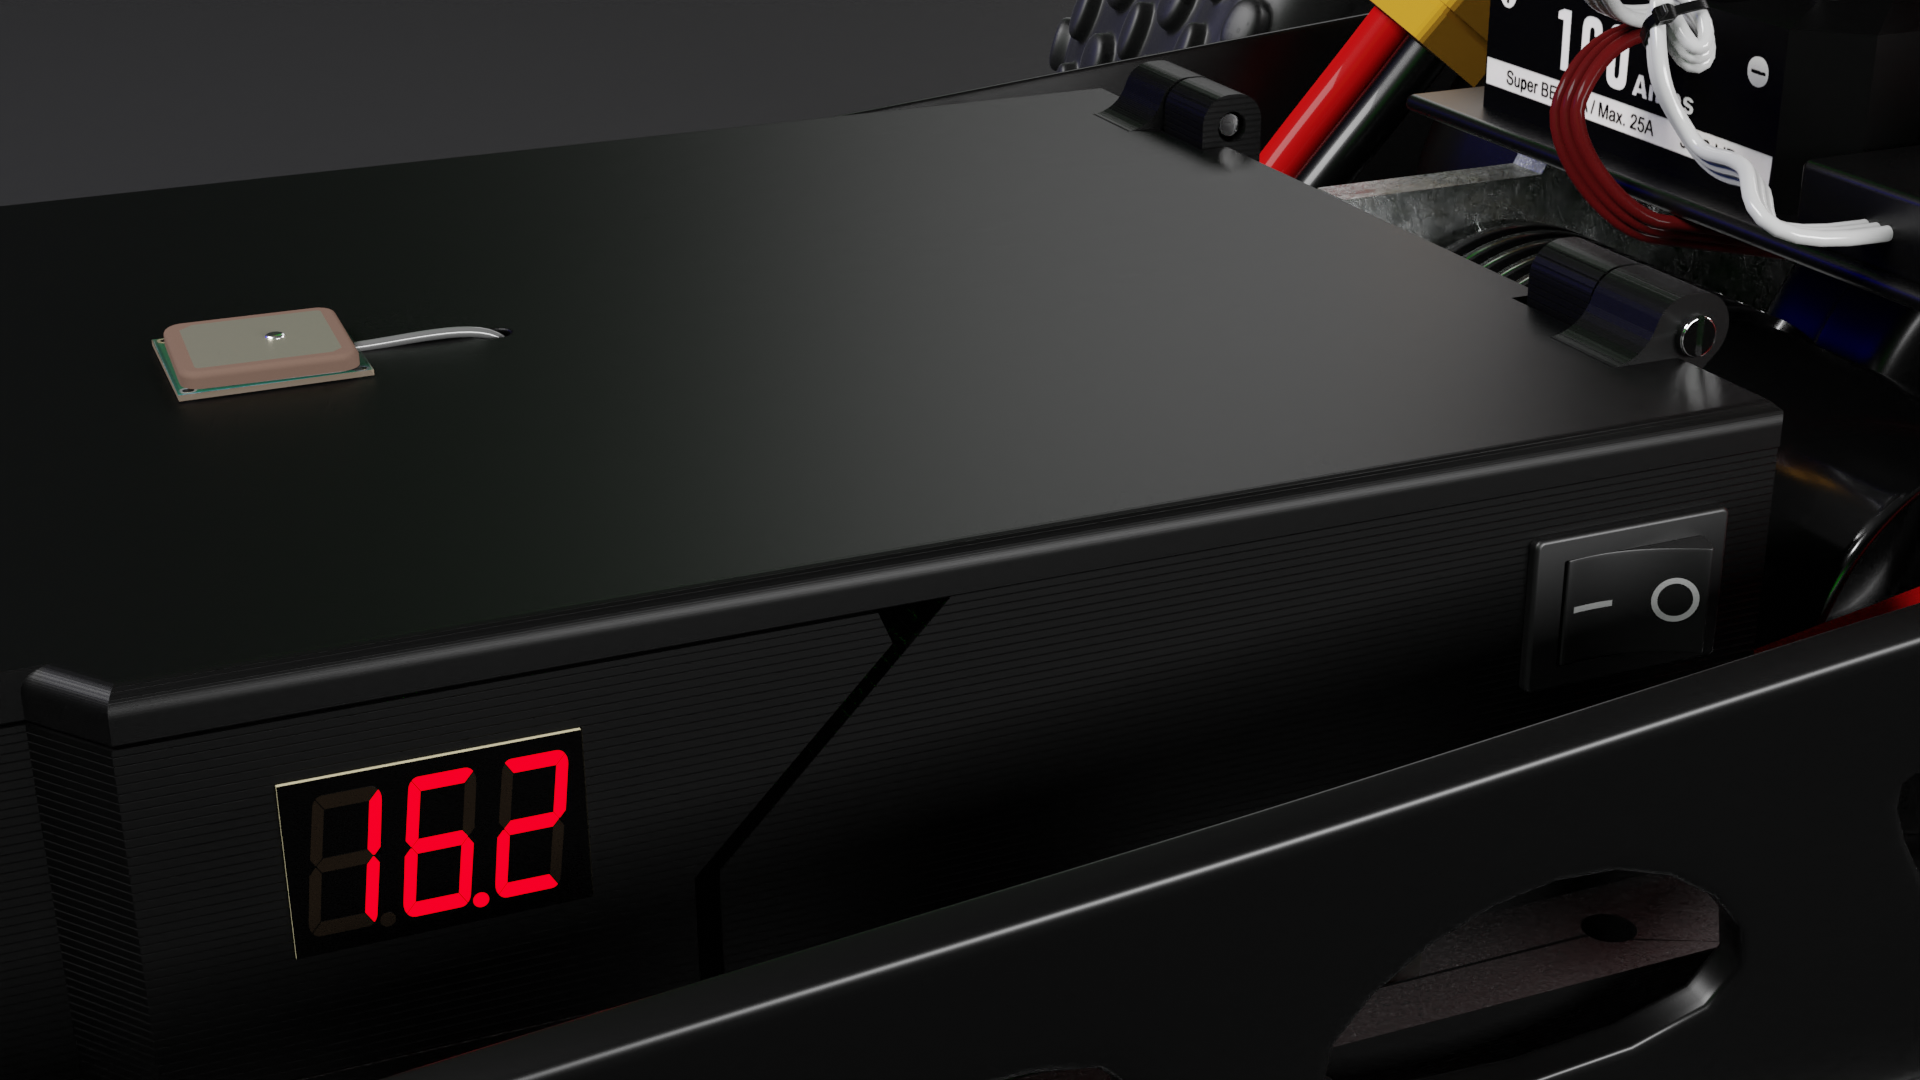
\includegraphics[scale=0.2]{switch.png}
\caption{7-Segmentanzeige und Kippschalter im Gehäuse}
\label{fig:switch}
\end{figure}

\subsection{Gehäuse}
\label{subsec:elekCasing}
Eine robuste, vielseitige Einhausung der Messelektronik ist essentiell, um diese stabil montieren sowie von äußeren Einflüssen wie Staub und Sand schützen zu können. Die Sitzkonstruktion des Autos wird entfernt, wodurch Raum für ein Gehäuse freigelegt wird. Als Basis dient eine einfache Plattform, welche an den ursprünglichen Montagestellen der Sitzkonstruktion in das Auto geschraubt wird. Direkt darunter, auf der Bodenplatte des Autos, befinden sich die Akkus. Auf diese Plattform werden mehrere Seitenwände aufgeschraubt.\\
Sämtliche Schraubverbindungen im und am Gehäuse werden mittels M3 Gewindeeinsätzen ermöglicht. Die \ac{FDM}-3D-gedruckten Gehäusekomponenten weisen Bohrungen auf, in welche diese Gewindeeinsätze eingeschmolzen werden. Diese Lösung, Schraubverbindungen in 3D-Druck-Komponenten zu ermöglichen, ist sehr belastbar und einfach umzusetzen, weshalb sie häufig eingesetzt wird. \\
Die U-förmige Rück- und gleichzeitig hintere Seitenwand, weist in Bodennähe eine rechteckige Ausnehmung auf, welche für die Durchführung der Versorgungsleitungen sowie den Sensorleitungen der hinteren Drehzahlsensoren vorgesehen ist. Auf der rechten Seite dieser Wand ist der Kippschalter der Versorgungsleitung eingefasst. Links befindet sich die \ac{USB}-A-Buchse für die Datenübertragung mittels \ac{USB}-Datenträger, wie es in Sektion \ref{subsec:Datenübertragungsmodus} näher beschrieben wird. An der hinteren Oberkante dieser Komponente sind außerdem zwei Scharniere ausgeführt, um den Deckel einfach öffnen und schließen zu können. Am vorderen Ende der Plattform ist links und rechts jeweils eine weitere Wandkonstruktion angebracht, welche mit der hinteren mit einem schmalen Abstand abschließt. Auf der rechten Wand befindet sich ein Taster für das Umschalten des Programmzustandes sowie eine \ac{RGB}-\ac{LED}, die diesen Zustand signalisiert. In der linken vorderen Wand ist die Siebensegmentanzeige eingebaut, welche die aktuelle Akkuspannung anzeigt. Diese vorderen Wandteile weisen außerdem eine Montagemöglichkeit für die Deckelverriegelungen auf. Der Deckel des Gehäuses deckt den gesamten Innenraum ab und kann durch die bereits erwähnten Scharniere auf- und zugeklappt werden. Mit Hilfe von zwei Drehverriegelungen wird der Deckel geschlossen gehalten. Wie in Sektion \ref{subsec:GPSmount} beschrieben, befindet sich im Deckel eine Bohrung für die Durchführung der GPS-Antennenleitung.\\
Um den Raspberry Pi und beispielsweise den Stepdown-Wandler auf der Grundplattform zu montieren, weist diese ebenfalls Bohrungen mit eingeschmolzenen Gewindeeinsätzen auf. Für die Montage sind außerdem einzelne Gehäuse für den Raspberry Pi und Stepdown-Wandler notwendig. Diese wurden mittels \ac{CAD} konstruiert und anschließend mit dem in Sektion \ref{subsec:tDUP} beschriebenen \ac{DUP}-Verfahren 3D-gedruckt. Da der Raspberry Pi Bohrungen in den Ecken aufweist, wird dieser mit M3 Schrauben in seinem Gehäuse montiert. Der Stepdown-Wandler hat keine Befestigungsbohrungen und wird deshalb mit doppelseitigem Klebeband befestigt. 

\subsection{Einbindung externer Elektronik}
\label{subsec:elekExtern}
Wie in Sektion \ref{subsec:RPMmount} bereits erklärt, sind die Drehzahlsensoren in der Nähe aller vier Räder angebracht. Eine zuverlässige Verbindung dieser Sensoren mit dem Raspberry Pi ist ausschlaggebend. Besonders bei den Vorderrädern, welche durch die Federung sowie die Lenkung Bewegungen ausführen ist eine robuste, aber flexible Verbindung zum Gehäuse notwendig. Aus diesem Grund werden als Verbindungselemente JST-XH Stecker und Buchsen verwendet und eine biegsame Mantelleitung zur Versorgung und Signalübertragung. Eine Mantelleitung hat den Vorteil, dass sie mehrere Adern mit einem Mantel umschließt, der es ermöglicht die Leitung stabil am Fahrgestell zu fixieren und die einzelnen Adern gegen mechanische Beanspruchung schützt. Auf diese Weise können die Sensoren außerdem an- und abgeschlossen werden.\\
Die insgesamt vier Mantelleitungen werden durch dementsprechende Ausnehmungen an den Gehäusewänden in das Innere des Gehäuses geführt. Um das Anschließen der Drehzahlsensoren zu vereinfachen, werden diese auf einer Anschlusskonstruktion mit mehreren JST-XH Buchsen angesteckt. Diese Buchsen sind bereits mit den korrekten Pins am Raspberry Pi verbunden. Auch das \ac{GPS}-Modul ist mit einer solchen Mantelleitung und JST-XH Verbindungen an dieser Anschlusseinheit angeschlossen.\\
Um den in Sektion \ref{subsec:Datenübertragungsmodus} beschriebenen Datenübertragungsmodus nutzen zu können, ist eine \ac{USB}-A-Buchse, welche von außerhalb des Gehäuses zugänglich sein muss, zu installieren. Diese von Außen zugängliche Buchse wird mithilfe eines micro-\ac{USB} auf \ac{USB}-A-Adapters, welcher an der Datenbuchse des Raspberry Pi angeschlossen ist, realisiert.